\subsection{K-Means}
There are many methods with which to segment data by clustering but K-Means is very popular for its simplicity and speed. Data points can belong in any one of K clusters whose average value is a centroid. Centroids may initially be randomly selected or be members of the given data set. 

Data points or samples are placed in the class of the centroid that is the closest, where the distance between them is the Euclidean Distance between their feature vectors as in \ref{eq:euclid}. 

\begin{equation}
    D(\vec{p},\vec{q}) = \sqrt{(p_1 - q_1)^2 + (p_2 - q_2)^2 +\hdots + (p_n - q_n)^2}
    \label{eq:euclid}
\end{equation} 

The algorithm that governs K-Means clustering is as follows:
    \begin{enumerate}
    \itemsep0em
        \item Place the initial K centroids.
        \item Assign all data points to their nearest centroid.
        \item Update the centroids' values to be the mean of all data points in their cluster.
        \item Repeat steps 2 and 3 until cluster centroids no longer move (converge) or until a desired number of iterations performed. 
    \end{enumerate}

K-means benefits greatly from its low computational cost to the point where often it is performed a number of times with different initial class centroids to yield a result with the smallest variance in each cluster. It suffers, however, from the implicit assumption that cluster sizes will be approximately the same. This is because the algorithm seeks to minimize variance (spread) in each cluster hence the \q{ideal} centroid placement will form distributions spherically about centroids. This method cannot disentangle overlapping samples from different classes. In Figure \ref{fig:clusters} approximately spherical clusters can be oberserved and the clear cutoffs between clusters ignores the class ambiguity of samples at the boundaries, this is called \emph{hard assignment}, as opposed to a \emph{soft assignment} that will consider the relative probabilities of a sample's class membership. 



\begin{figure}[H]
    \centering
    \centering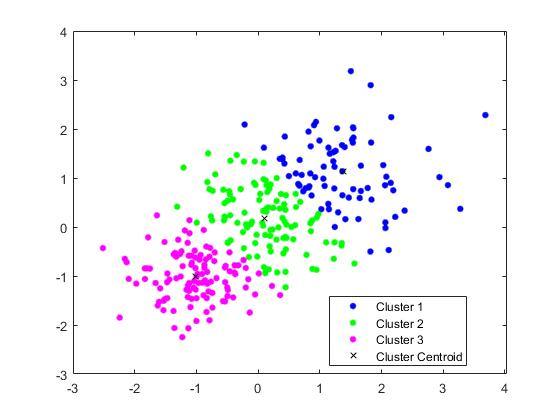
\includegraphics[width=300pt]{kmeans_clusters}
    \caption{K-Means clustering performed on random data.}
    \label{fig:clusters}
\end{figure} 